\chapter{Support Vector Machines}
\label{ch:svm}

Support vector machines (SVM) are another example of linear classifiers, similar to logistic or linear regression. However, SVM can overcome splitting the data by a plane by using the so-called \textit{kernel trick}. This means the hyperplane (decision boundary) can be transformed to a higher-dimensional space, which can fit the data nicely. In such a way, SVM becomes a non-linear classifier and can fit more complex data sets.

\begin{marginfigure}
    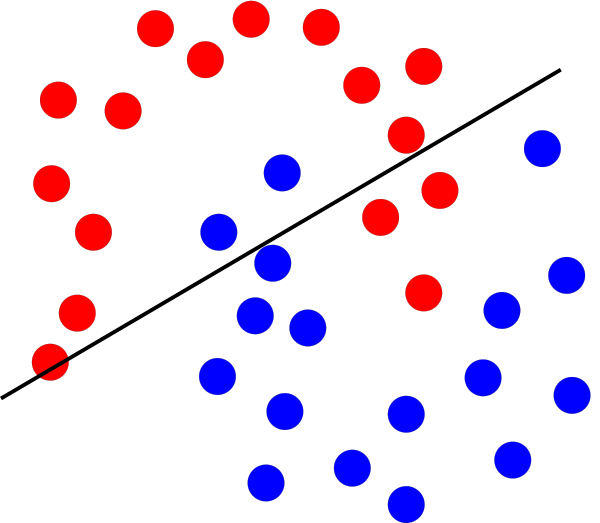
\includegraphics[width=50mm]{linear-regression.png}%
    \caption{Decision boundary of a linear regression classifier.}
  \end{marginfigure}

\begin{marginfigure}
    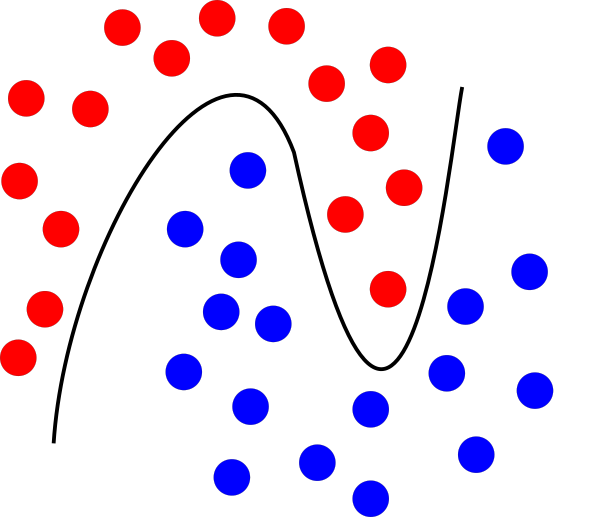
\includegraphics[width=50mm]{svm.png}%
    \caption{Decision boundary of a support vector machine classifier with an RBF kernel.}
\end{marginfigure}

The magic of SVM (and other methods that can use kernels, and are thus called kernel methods) is that they will implicitly find a transformation into a (usually infinite-dimensional) space, in which the distances between objects are such as prescribed by the kernel, and draw a hyperplane in this space.

\begin{figure}[h]
    \centering
    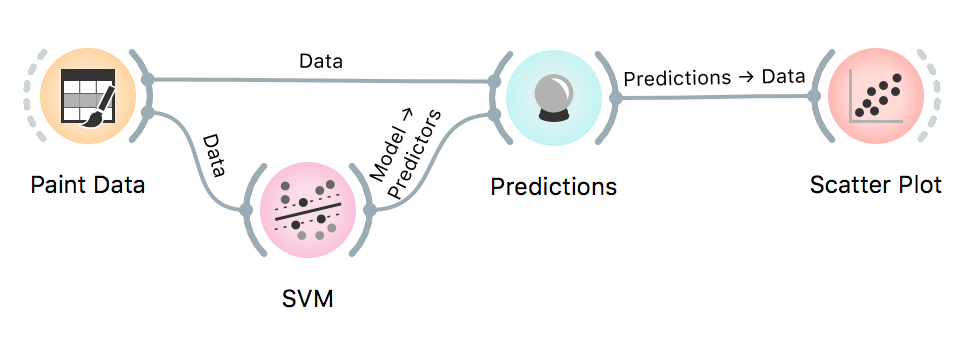
\includegraphics[scale=0.5]{workflow.png}
    \caption{$\;$}
\end{figure}

Abstract talking aside, SVM with different kernels can split the data not by ordinary hyperplanes, but with more complex curves. The complexity of the curve is decided by the kernel type and by the arguments given to the algorithm, like the degree and coefficients, and the penalty for misclassifications.

\begin{figure}[h]
    \centering
    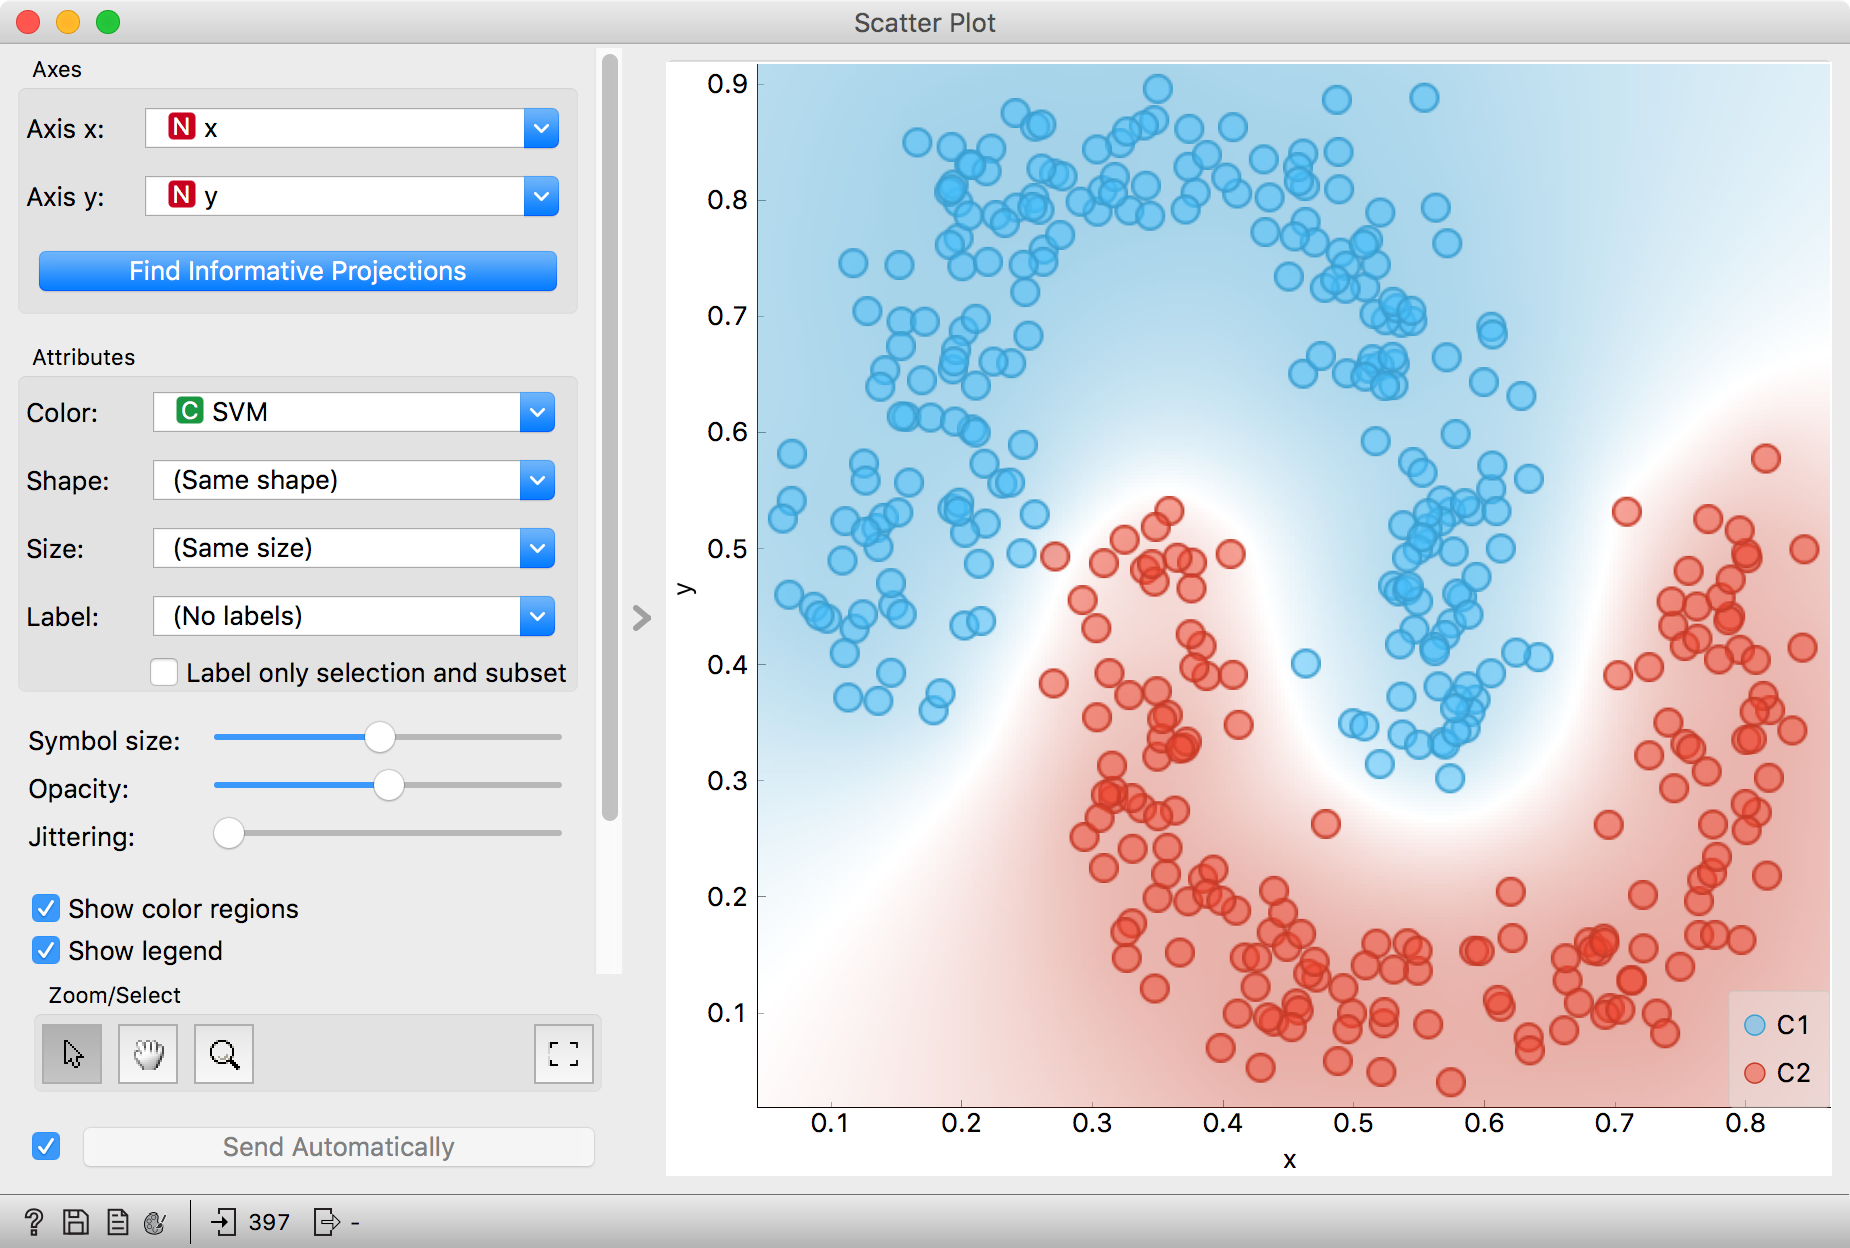
\includegraphics[height=70mm]{svm-orange.png}
    \caption{$\;$}
\end{figure}
